% paper/figures/latex_includes.tex
% Include these blocks at the corresponding Results locations.
\begin{figure*}[t]
  \centering
  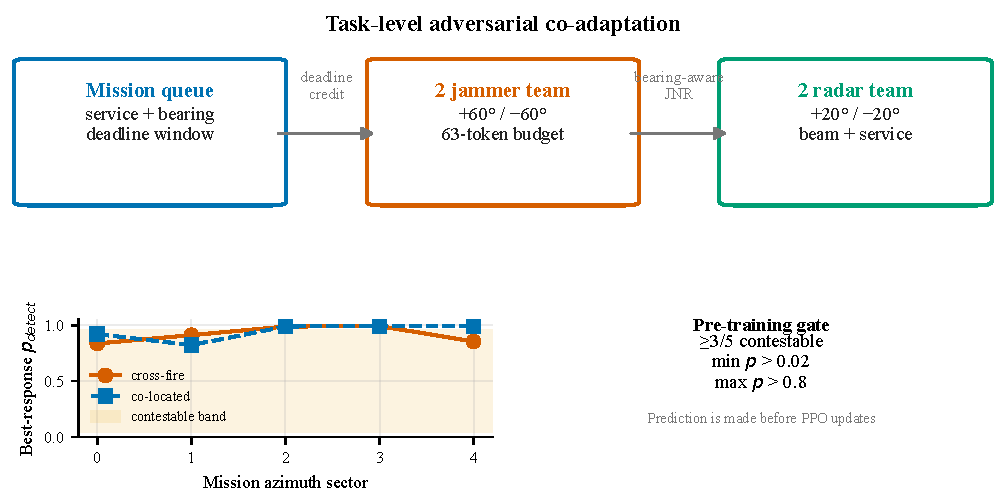
\includegraphics[width=0.96\textwidth]{figures/fig1_benchmark_anatomy.pdf}
  \caption{FluxPhased couples deadline-constrained mission tracking to
  bearing-aware jammer--radar link physics. The lower panels show the
  pre-training best-response detection profiles for the cross-fire and
  co-located controls; the shaded interval is the contestability band.}
  \label{fig:benchmark}
\end{figure*}

\begin{figure}[t]
  \centering
  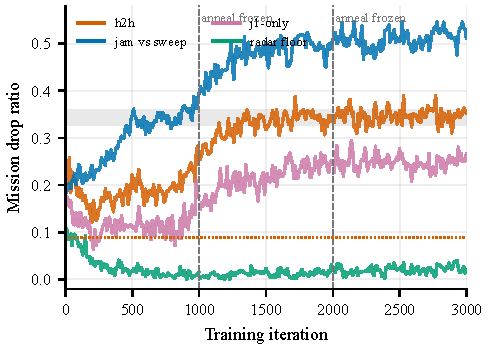
\includegraphics[width=\columnwidth]{figures/fig2_training_curves.pdf}
  \caption{Three-stage S7 training trajectory for seed 20260801. The two
  dashed lines mark continuation boundaries at iterations 1000 and 2000;
  entropy is frozen during both continuation stages. The final 2000--3000
  region is stationary across all four views.}
  \label{fig:training}
\end{figure}

\begin{figure}[t]
  \centering
  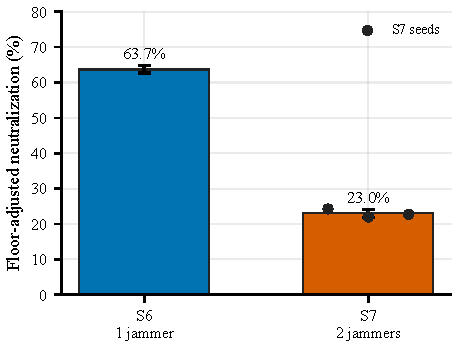
\includegraphics[width=\columnwidth]{figures/fig3_neutralization.pdf}
  \caption{Floor-adjusted defense neutralization falls from
  $63.7\%\pm1.0\%$ in S6 to $23.0\%\pm1.1\%$ in S7. Black points show the
  three S7 training seeds; bars show the aggregate mean and standard
  deviation.}
  \label{fig:neutralization}
\end{figure}

\begin{figure*}[t]
  \centering
  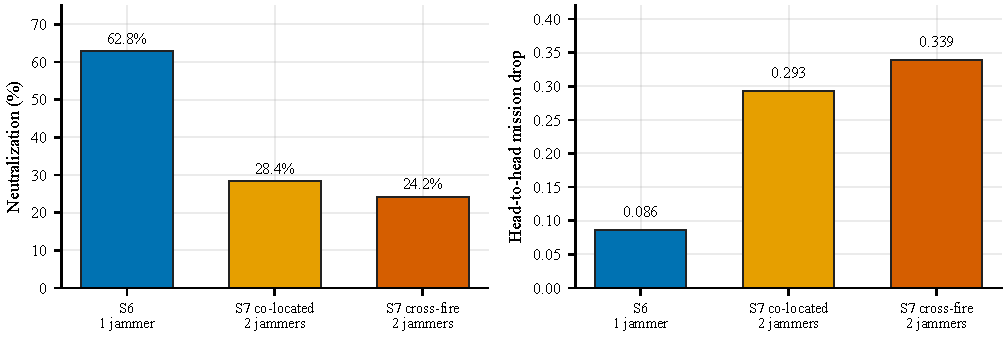
\includegraphics[width=0.96\textwidth]{figures/fig4_mechanism_ablation.pdf}
  \caption{Mechanism decomposition. Two co-located jammers already reduce
  containment relative to S6; cross-fire geometry adds a smaller, directional
  penalty. The two panels report neutralization and head-to-head mission drop
  under matched task, budget, and training protocols.}
  \label{fig:ablation}
\end{figure*}

\begin{figure*}[t]
  \centering
  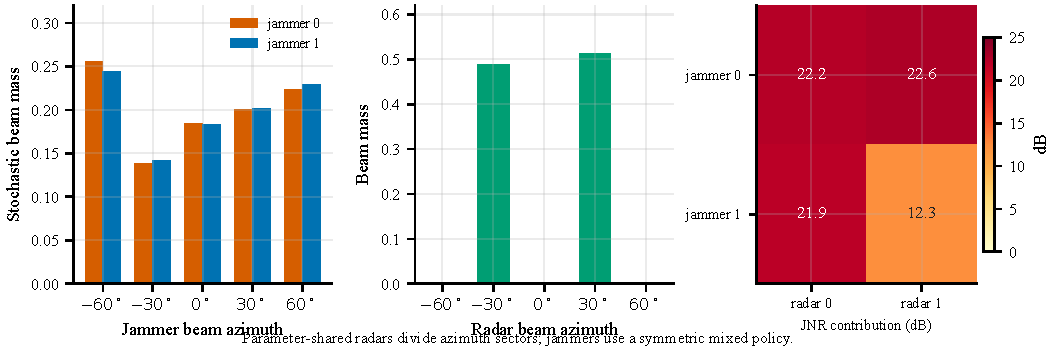
\includegraphics[width=0.96\textwidth]{figures/fig5_behavior.pdf}
  \caption{Equilibrium behavior at the converged S7 checkpoint. The radar
  team divides the mission plane between azimuths near $-30^\circ$ and
  $+30^\circ$, while the jammer team uses a symmetric mixed beam policy. The
  heat map reports active-only pairwise JNR contributions in dB.}
  \label{fig:behavior}
\end{figure*}

\begin{figure}[t]
  \centering
  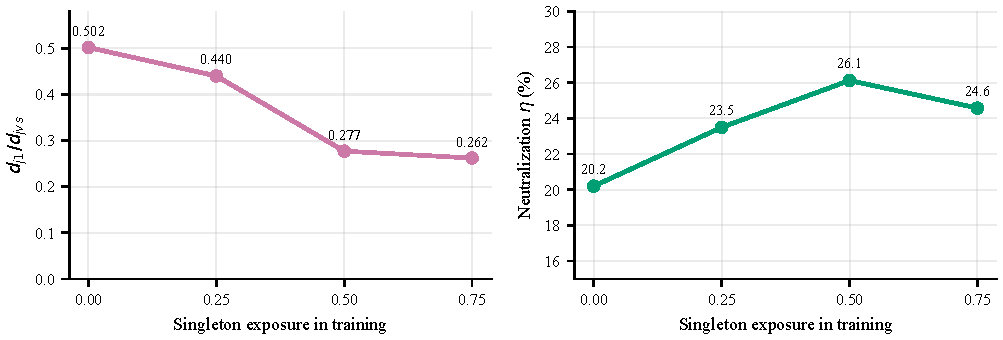
\includegraphics[width=\columnwidth]{figures/fig6_r5_dose_response.pdf}
  \caption{R5-lite opponent-class mixing. Singleton relative leverage
  $d_{j1}/d_{jvs}$ decreases from 0.502 to 0.262 as singleton exposure rises;
  neutralization improves from 20.2\% to a maximum of 26.1\% at 50\%
  exposure. Absolute drops are confounded by skipped jammer updates.}
  \label{fig:r5}
\end{figure}
